
\subsection{Generic Local Search}
1) An initial solution s\newline
2) N(s) is the neighborhood of s\newline
3) Some moves are legal (satisfy the constrains) some arn't : L(N(s),s) is the set of legal moves from a solution s.\newline
4) S selects the move in the legal moves


\begin{figure}[!ht]
    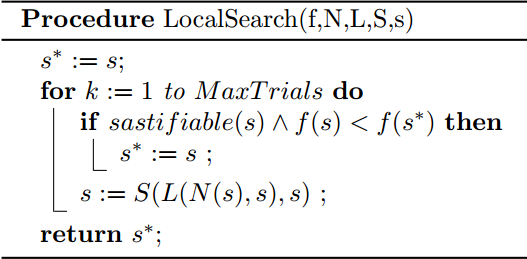
\includegraphics[width=0.4\linewidth]{LocalSearchGenericAlgo.png}
    \label{fig:Knapsack_example}
\end{figure}
\FloatBarrier
 

\subsection{Improvement Heuristic}
We can improve this algorithm with two heuristics:\newline
\textbf{L-Improvement} will only accept moves that improve the solution\newline
\textbf{S-Best} will select one on the move randomely in case of tie.\newline

\subsection{Local Minima}

A big problem with local search is that you can be stuck in a local minima(maxima) for a minimization problem(maximimzation).\newline

We have two solutions for that:\newline
1)We can accept to degrade the solution\newline
2)Enlarge the neighborhood\newline

\subsection{Sudoku exemple}
There is two type of constraints : Hard and Soft.\newline
\textbf{Hard Constraints} much be respected at all time during the local search.(They are enforced at initialization)
\textbf{Soft Contstraints} are the constraints that can be violated during the search in order  to find better solutions.\newline

For the sudoku exemple we execute swaps between cases to try to lower the number of soft constraints violated.

Adding more constraints in the hard constrains makes the initialization harder but makes the local search process easier.

\subsection{OscarR CBLS}
\textbf{OscarR CBLS} is a library for local search.
You add the constraints and the objectifs function and it will compute the violations and the delta's for you.

With this you can focus more on the search process(moves and meta-heuristics).

\subsection{Tabu Meta Heuristic}
\textbf{Tabu meta heuristic} accept to degrade the solution in order to get out of the local minimas.\newline

Whenever you perform a move, this move becomes tabu for a certain duration(number of iteration).When you are stuck in a local minima the algrithm keeps iterating between a couple of moves without finding a better solution. By making a move tabu you force it to chose some other point and escape from the  local minima.\newline

If your neightboord is connected and you let the tabu search run indefinatly with a long enought tabu periode your algorithm will end up finding the optimal solution

\subsubsection{Improvement on tabu search}
Aspiration\newline
You not only consider the non tabu moves but you also considere the best tabu moves if they improve your best solution.
You might have use a certain move to get out of a minima at some point and escape from this local minima. But after that maybe the move is still tabu but alows you to find a better solution that the one you have found so far. Aspiration allows you to find this better solution even tought the move is in the tabu list.

Restart\newline
Every X iteration you change randomely some variables in you current solution and you restart the from that point. This allows you to travel further in the search space in order to maybe find a better solution far from the position you were before.

\subsection{Connected Neighborhood}
A neighborhood is connected if and only if for each
solution s, there exists a path to an optimal solution s*.

This means that if you make the right moves, your neighboord is large enought to find the optimal solution. However having a connected neighboord doens't means you will find the optimal solution(in case you don't make the right moves because of a bad heuristic for instance).\newline

with a connected Neightboord you are not forced to restart(even thought this can improve the time to find the best solution).
Also you can find the solution find a random heuristic.

\subsection{Lin-Kernighan algorithm}
In a TSP, 2-opt is an algorithm that swap 2 edges.
3-opt is the algorithm that swap 3 edges, 4-opt..
Obviouly there is more 3 opt moves than 2 opt move and more 4 opt moves than 3 opt moves...
Above a 4-opt the neighboord is getting way too big.
This is why we can limit ourself to \textbf{Sequential k-Opt moves}.
A k-Opt move is called sequential if it can be described
by a path alternating between deleted and added
edges.

We want to greedily build a Kk-opt move(maybe not THE best move in the k-opt neighboord).
We will start this algorithm with different k's and use the one that gives use to most gain.

This algorithm is the Lin-Kernighan.
We build a set X and Y of edges such that X are the deleted edges and Y are the added edges
Those edges are added elements by elements(empty at start).
We could start the algirthm just like that but we don't want it to run forever. This is why we add some criteria to make is sufficiently efficient.\newline

The sequential exchange criterion\newline
There can not be two added edges in a row. There must be an added edge folowed by a deleted edge.
The feasibility criterion\newline
The resulting configuration must be a cycle.
The positive gain criterion\newline
We chose the set Y of edge so that we gain from the nex configuration(If the changes gives us a worst solution than the one we had before it is not interresting)
The disjunctivity criterion\newline
X and Y disjoint(You can't add a deleted edge or you can't delete an added edge.
The candidate set criterion\newline
When looking for a new edge in Y we limit ourself to only considere the 5 nearest neighbors of the vertice.\newline

\subsection{ATSP reduction to TSP}
ATSP = Asymetric traveler salesman problem.
This means that the weight of the edge from A to B isn't neceseraly the same as the one from B to A. To reduce this problem to the simple TSP we double every every vertice and put an -inf weight to it.\newline

\subsection{Vehicule Routing Problem}
This a local search problem mixing the bin packing problem and the TSP problem.
We have two types of initializations for this local search.\newline
\subsubsection{Saving Heuristics}
We start with a single vehicule for each customer we need to serve.
Afterthat we merge routes to decresae the total distance the most without exceeding the capacity.We do that iteratively until no more routes can be merge withtout violating the capa constraints\newline

\subsubsection{Sweep Heuristic}
Westart with a ray centered at the depot.We start the turn the ray around the depot and every time we cross a customer with the ray we add it to the current cluster. If the nest customer exceed the capacity we start a new cluster.\newline

\subsection{Scheduling moves}
We have a set of activities that can not be interrupted and that have a certain length and a certain ressource need.
The ressource capacity is C.
How to minimize the total duration withtou exceeding the total capcity.\newline
We can use the IFlat-IRelax algorithm(Local search algorithm).\newline
We iterativelay flatten then Relax.\newline
1)\textbf{Flatten} : We add strong percedences constraints until the capcity constrains is satisfied.
2)\textbf{Relax} : We remove some precedences randomely on the critical path(the critical path is that path that is the longest in the schedule(the one that makes the schedule the longer)

\subsection{Eternity II}
16x16 edge matching puzzle.\newline
What neightborhood should we chose?\newline
Remove m pieces from non edge adjacent positions(up to $n^2/2$ ) and remplace them optimally. \newline
Exemple : We remove 5 edges and check for every single on of those pieces the number of correct adjacent edges it gives us. We have a complete weighted bipartite graph beteen the removed piecs and holes that we can solve thanks to a maximum assignement problem.
The size of the Neighborhood is exponential but it can be optimally explored in polynomial time.(Hungarian algorithm O(m³).
